\cotefile{12}
\scanpage{82}
$C$ courbe lisse \inserted{propre} sur $\mathbb{F}_{\unsure{q|p}}$

$A$ schéma abélien sur $C$.

Des conjectures de Weil, résulte que
\[
H^i(C,A)=0\qquad\text{si}\quad i\geq 2
\]
et sans doute, utilisant Tate, on doit avoir
\[
H^1(C,A)=0
\]

Soit $x$ un pt fermé de $C$, $U=C-\{x\}$, alors on a
\diagram{\scriptsize
\begin{tikzcd}[ampersand replacement=\&,column sep=.65em,row sep=.35em]
\deleted{\unsure{H^0(U,A)|H^0(C,A)}}\arrow[r] \&
\deleted{\unsure{H^1_x(C,A)}}\arrow[r] \&
H^1(C,A)\arrow[r] \& H^1(U,A)\arrow[r] \& H^2_x(C,A)\arrow[r] \& H^2(C,A)\\
\& \deleted{\unsure{0}} \& \shortparallel \& \& \& \shortparallel\\
\& \& 0 \& \& \& 0
\end{tikzcd}}
d'où
\[
H^1(U,A)\simeq H^2_x(C,A)
\]
Or par Tate,
\[
H^2_x(C,A)\deleted{\unsure{\simeq|=}}\;H^1(K_x,A)\deleted{\unsure{\simeq|=}}\quad
\text{\uline{dual} de }H^0(K_x,A^{*})\deleted{\unsure{\simeq}}
\]
\deleted{\unsure{ce|on} \unsure{n'est en général pas un} \unsure{groupe|groupe fini}\inserted{\unsure{groupe de}}} \uuline{c'est donc essentiellement un $p$-\deleted{\unsure{fini}}groupe}, modulo groupe fini ! O.K.

Peut se généraliser au cas où on prend $X$ régulier dont on enlève un diviseur régulier \textendash\,\textendash\,\textendash\,\textendash
% archive sheet number: 81
\scanpage{84}
\uline{Calculs} pour $T_\ell(G_m)\inserted{=\mathbb{Q}_\ell(1)}$ et $G_m$.

$X$ de type fini sur $\mathbb{Z}$

\[
\begin{aligned}
H^0(X,\mathbb{Q}_\ell(1))\deleted{\unsure{\otimes G_m)}}&=0\\
H^1(X,\mathbb{Q}_\ell(1))&=\tikz[baseline=(a.base)]{\node[draw,ellipse,inner sep=1pt] (a) {$H^0(X,O_X^*)\otimes_{\mathbb{Z}}\mathbb{Q}_\ell$};}\\
H^2(X,\mathbb{Q}_\ell(1))&\quad\text{extension de }\,
\tikz[baseline=(b.base)]{\node[draw,rounded corners,inner sep=2pt] (b) {$T_\ell(H^2(X,G_m))$};\draw (b.north east) .. controls +(.13,.22) and +(-.18,-.04) .. ++(.55,.24);}
\quad\text{par}\\
&\hspace{4em}\tikz[baseline=(c.base)]{\node[ellipse,draw,inner sep=1pt] (c) {$\deleted{\unsure{R}}H^1(X,\unsure{\underline{O}_X^*|O_X^*|\mathcal{O}_X^*})\otimes\mathbb{Q}_\ell$};}
\end{aligned}
\]
\margin{\uline{coBrauer}}
$H^3(X,\mathbb{Q}_\ell(1))\simeq T_\ell(H^3(X,G_m))$ est ce qu'il peut [p. ex. $\mathbb{Z}_\ell$ si $X$ \deleted{\unsure{modèle}}modèle can. d'un corps de fonctions d'une variable sur $\mathbb{F}_p$]
\[
\begin{aligned}
H^i(X,\mathbb{Q}_\ell(1))&=0\qquad\text{si}\quad i\geq4\qquad ??\\
\shortparallel&\\
T_\ell(H^i(X,G_m))&
\end{aligned}
\]

On conjecture (Artin) que $H^2(X,G_m)={}\text{groupe fini}$ si $X$ propre sur $\mathbb{Z}$. \deleted{Mais si} \inserted{Vrai} si $X$ courbe projective lisse sur $\mathbb{F}_p$, mais faux quand on lui enlève des pts \textendash\ le rang du $H^2$ augmente d'autant

$H^3(X,\mathbb{Q}_\ell(1))$ : quel est sa taille [il décroît en passant à un ouvert de $X$]
% archive sheet number: 83
\scanpage{86}
\mspage{17}\uline{Formes positives}

Le \unsure{théor.|thème|théorie} étant géométrique, nous nous plaçons sur un corps alg. clos $k$. Nous ne considérons que les motifs $1/2$ \uline{simples} sur $k$, \inserted{purs,} de poids $p$. Soit $M$ un tel motif, considérons les formes
\[
M\times M\longrightarrow\mathbb{Q}(-p)
\]
i.e. les éléments de
\[
\Gamma_k\bigl(\mathscr{H}om(M\otimes M,\mathbb{Q}(-p))\bigr)
=\unsure{\Phi|\mathscr{L}|\mathcal{L}}(M)
\]
où le \deleted{\unsure{$\Gamma_k$ est}} $\mathscr{H}om$ est bien de poids $0$. Elles forment un vectoriel de \deleted{poids \unsure{0}}\inserted{dim finie} sur $\mathbb{Q}$. On considère le \inserted{sous-}espace \deleted{des} \deleted{\unsure{formé}} des formes \uline{symétriques} si $p$ pair, \uline{alternées} si $p$ impair. Cet espace sera noté $\Phi^s(M)$. Noter les hom canoniques
\[
\Phi^s(M)\otimes\Phi^s(N)\unsure{\longrightarrow|\mathbin{-}}\Phi^s(M\otimes N)
\]
% archive sheet number: 85
\scanpage{87}
par produit tensoriel \unsure{des|de} formes [N.B. le produit tensoriel de deux formes \deleted{symétriques, ou de} de $=$ type de symétrie est symétrique \textendash\ de deux types opposés de symétrie est antisymétrique]. Bien entendu, ils ne sont pas en général bijectifs (mais du moins injectifs).

On a aussi
\[
\unsure{\Phi|\mathscr{L}|\mathcal{L}}^s(M'\times M'')\simeq
\Phi^s(M')\times\Phi^s(M'')\times B(M',M'')
\]
où
\[
B(M',M'')=\operatorname{Hom}(M'\otimes M'',\mathbb{Q}(p)).
\]

Ceci posé, on \deleted{veut pour \unsure{dt|tt}} \inserted{a dans} tt $\Phi^s(M)$ un cône \inserted{convexe} \deleted{\unsure{f}}fermé $\Phi^+(M)$.

On a les propriétés suivantes :

(i) $\Phi^+(M)$ a un intérieur non vide.

(ii) Un élément de $\Phi^+(M)$ est dans l'int. de $\Phi^+(M)$ ssi il est non dég.

\margin{formes $\in\Phi^+(M)$ sont dites pseudo-amples, celles dans l'intérieur sont dites \uline{amples}}
% slanted

(iii) Pour $M\to N$, $\Phi^+(N)$ s'envoie dans $\Phi^{\unsure{+|e}}(M)$.

(iv) \deleted{\unsure{(iii)} \unsure{Pour}} Si $M\longrightarrow N$ injectif, \deleted{\(\Phi^+(N)\)} l'intérieur de $\Phi^+(N)$ s'envoie dans l'intérieur de $\Phi^+(M)$ (formes amples $\longrightarrow$ formes amples)
% archive sheet number: 86
\scanpage{88}
\deleted{\unsure{(iii)}} \deleted{\unsure{(iv)|(v)}} i.e. la forme induite sur $M$ \inserted{par une forme ample} est non dégénérée, donc $N=M\oplus M^\perp$, et la forme sur $N$ est la somme des formes induites sur $M,M^\perp$.

(v) La somme directe de deux formes \deleted{positives \unsure{ou}} pseudoamples (amples) est itou.

(vi) Le produit tensoriel de deux formes amples est ample.

(vii) Si $p=0$, de sorte que \unsure{essentiellt|essentielt|essentiellement} $M$ est défini par un vectoriel de dim finie sur $\mathbb{Q}$, alors les formes amples sont les formes \uline{définies positives}. \deleted{\unsure{Plus généralement|Plus généralemt} pour $M. (p)$, $M$ un vectoriel de dim finie sur $\mathbb{Q}$ ; utilisant l'isom canon}

(viii) Cas de $\mathbb{Q}(p)$ : on a $\unsure{\Phi|\mathscr{L}|\mathcal{L}}^s(\mathbb{Q}(p))\simeq\mathbb{Q}$, et on veut que les formes amples correspondent aux nbs \inserted{\uline{\unsure{strictt|strict\textsuperscript{t}|strictement}}} \uline{positifs}.
% archive sheet number: 87
\scanpage{89}
De (vi) et (viii) résulte que pour tt motif $M$ et entier $n$, l'isomorphisme
\[
\unsure{\Phi|\mathscr{L}|\mathcal{L}}^s(M)\simeq\deleted{\unsure{M}}\Phi^s(M(n))
\]
est compatible avec les cônes amples.

De (iv) et (vi) résulte que si $p=0$, une forme ample sur $M$ induit une forme \uline{définie positive}
\[
\Gamma_k M\times\Gamma_k M\unsure{\mathbin{-}|\longrightarrow}\Gamma_k\mathbb{Q}(0)=\mathbb{Q}
\]

Si on décompose $M$ (de poids $p$) en composantes isotypiques $M_\alpha$, il vient
\[
\Phi^s(M)\simeq\mathop{\deleted{\unsure{\sum}}\unsure{\bigoplus|\prod}}\limits_\alpha\Phi^s(M_\alpha)
\]
donc pour étudier les formes positives, il suffit de les étudier en principe sur \unsure{des|les} morceaux isotypiques, qui sont d'ailleurs de la forme
\[
I\otimes_A\deleted{\unsure{M|N}}V
\]
où $I$ est un motif simple, $A$ son anneau des endomorphismes, qui est un corps, et $\deleted{M}V$ un \uline{vectoriel} sur $A$
% archive sheet number: 88
\scanpage{90}
\mspage{18}
\uuline{Dictionnaire}\qquad Fonctions L \textendash\ \unsure{Chronologie|Cohomologie|Chronologique} à action galoisienne.

Soit $k$ un \deleted{corps ou} anneau

\deleted{\unsure{\(M\)|\(A\)} la catégorie} \deleted{$\operatorname{Mod}(\mathbb{Z})$ la catégorie} $C$ la catégorie des modules de longueur finie sur $k[t]$ $=$ \deleted{\unsure{vectoriels}}\inserted{modules} $V$ \inserted{proj.} de \deleted{dim}\inserted{rang} fini sur $k$ muni d'un endomorphisme $f$ $=$ $k[\deleted{\unsure{\mathbb{Z}}}\mathbb{N}]$-modules, \inserted{projectifs} de \deleted{\unsure{rang|de type}} finie sur $\deleted{\unsure{V}}k$.

Cette catégorie donne lieu à un $\lambda$-anneau, noté $R^{\unsure{\bullet|\cdot}}(\deleted{\unsure{\mathbb{Z}}}\mathbb{N};k)$, qui est aussi, \inserted{si $k$ est un corps,} le \deleted{$\lambda$-anneau} \inserted{groupe} libre engendré par les classes des \deleted{\unsure{\(V\)}}$k[\deleted{\unsure{\mathbb{Z}}}\mathbb{N}]$-modules simples \inserted{finis sur $k$}, ou avec les $k[t]$-modules simples, ou avec les polynômes \inserted{unitaires} irréductibles $P\in k[t]$, en associant à $P$ le module $k[t]/Pk[t]$. À tout tel $P$ \inserted{$k$ \deleted{\unsure{un}} corps ou non}, \inserted{est} associé à un $(V,f)$, dont le polynôme car. est précisément $P$,
\[
P(t)=\det(t\,\mathrm{id}-f)
\]
[vrai pour tt $P$, irréd. ou non !]. Il nous sera plus commode de remplacer $P(t)$ par
\[
Q(t)=t^dP\left(\frac{1}{t}\right)=\det(1-tf)
\]
qui est un polynôme quelconque à coeff. cst égal : $1$.
% archive sheet number: 89
\scanpage{91}
Ainsi, on obtient via le pol. car. modifié un hom
\[
(V,f)\longmapsto\frac{1}{\det(\mathrm{id}_V-ft)}=L(\unsure{V|N},f)
\]
\[
R(\deleted{\unsure{\mathbb{Z}}}\mathbb{N};k)\longrightarrow 1+k[[t]]^+
\]
\margin{en fait, à valeurs \unsure{ds|dans} les \uline{fonctions rationnelles} de valeur $1$ en $0$}
qui \inserted{(composé avec l'\deleted{\unsure{involution|antiautomorphisme}}\inserted{aut} ``additif'' $\varphi(t)\longmapsto\frac{1}{\varphi(t)}$ dans $1+k[[t]]^+$)} est un hom de $\lambda$-anneaux,

Lorsque $k$ est \unsure{un|\deleted{un}} corps, l'hom précédent est injectif. En effet, \deleted{si} \deleted{$k$ est alg. clos,} la connaissance de la série formelle permet de reconstituer \inserted{la fonction rationnelle} \inserted{\unsure{donc}} [$k[t]$ étant factoriel.] l'élément $\sum_{\substack{P\ \mathrm{pol.}\\\text{unitaire}}}c_P(V_P,f_P)$ \deleted{dont} par
\[
L=\prod_Q Q^{c_P}
\]
[$Q$ et $P$ associés de la façon précisée plus haut].

Notons qu'on a un homomorphisme naturel \deleted{\unsure{le groupe log}}
\[
\begin{aligned}
1+k[[\unsure{1|t}]]^+&\longrightarrow k[[t]]\\
\varphi(t)&\longmapsto\frac{\varphi'(t)}{\varphi(t)}\deleted{\unsure{=}}
\end{aligned}
\]
qui correspond à
\[
\Lambda(V,f)(t)=\frac{L(V,f)'(t)}{L(V,f)(t)}
=\bigl[\log L(V,f)\bigr]'=\frac{1}{t}\sum_{1}^{\infty}(\operatorname{Tr}f^n)t^n.
\]
\deleted{\unsure{En car. 0, on peut|En car. 0, on}} Si $k$ de car. $0$, \inserted{i.e. $k\supset\mathbb{Q}$} on peut inverser cet homomorphisme par $\exp\bigl(\int_0^{\deleted{\unsure{t}}\ldots}\Lambda(V,f)(t)\bigr)$. Donc \inserted{si $k$ est} \inserted{un corps de car. $0$,}
\[
\Lambda:R(\mathbb{N},k)\longrightarrow k[[t]]
\]
est alors injectif \deleted{($k$ corps}
% archive sheet number: 90
\scanpage{92}
Si $k$ n'est pas de car. $0$, on ne peut en général aller en sens inverse, et $R(\mathbb{N},k)\xrightarrow{\Lambda}k[[t]]$ n'est \deleted{en général} pas injectif, [$k$ corps de car $>0$]

\medskip\centerline{\rule{2.6em}{0.3pt}}\medskip

On voit \deleted{que} par la formule de Lefschetz-Weil-Grothendieck que la connaissance de la fonction $L$ de $(X,F$ \deleted{\unsure{sur}}compactifiable sur $\mathbb{F}_p$, \inserted{à coeff. dans $F$,} \uline{équivaut} à celle de l'élément
\[
\underline{\chi}(F)=\sum(-1)^i\,\mathrm{cl}\,H^i_!(\overline{X},\overline{F})
\quad\text{de}\quad R(\mathbb{N},\mathbb{Q}_\ell)
\]
[car \unsure{essentiellt|essentiellement} cette fonction $L$ est l'image de $\underline{\chi}(F)$ dans $1+\mathbb{Q}_\ell[[t]]^+$].. Lorsque on admet les conjectures de Weil, et $F$ \inserted{est un motif,} $\underline{\chi}(F)$ se décompose suivant des poids en des $\sum(-1)^i\deleted{\unsure{\underline{\chi}}}\underline{h}^i_{\unsure{!}}(F)$, $\underline{h}^i(F)\in R(\mathbb{N},\mathbb{Q}_\ell)$, et la \deleted{\unsure{conna|connaissance}}connaissance de $L(X,F)(t)$ \uline{équivaut} à celle des $\underline{h}^i(F)$ : les $\underline{h}^i(F)$ correspondent à la décomposition de $L(X,F)$
% archive sheet number: 91
\scanpage{93}
\deleted{\unsure{suiv.|facteurs}} en groupant suivant les valeurs absolues des zéros et pôles \ldots . Lorsque $X$ est complet et lisse, \inserted{et $F$ \unsure{constant tordu|localement tordu|localement constant}, de poids $p$,} on a $\underline{h}^i(F)=H^{i-p}(\overline X,\overline F)$ comme $\mathbb N$-modules, dans ce cas la connaissance de $L(X,F)$ équivaut à celle des $H^{i\deleted{\unsure{-q|-p|-\rho}}}(\overline X,\overline F)$ et l'opération du frobénius dedans.

\diagram{\begin{tikzcd}[ampersand replacement=\&,column sep=2em,execute at end picture={\draw (current bounding box.south west) -- (current bounding box.north east);\draw (current bounding box.north west) -- (current bounding box.south east);}]
\deleted{X}\arrow[r,dash]\arrow[d,"\deleted{\unsure{f}}"'] \& \deleted{X_{\unsure{\eta|K}}}\arrow[d,dash]\\
\deleted{Y}\arrow[r,dash] \& \deleted{K=\text{corps des fonctions de }Y}
\end{tikzcd}}
\deleted{Soit $f:X\mathbin{-}Y$ morphisme [\unsure{lisse|disons} propre] avec $X,Y$ \unsure{compactifiables|simplifiables} de type fini sur $\mathbb F_p$. Considérons les ouverts denses $U$ de $Y$, et les $L(f^{-1}(U),F)$. Pour $U$ variable, ces fonctions rationnelles}

Considérons d'autre part \inserted{[pour $X$ de dim $n$]} les ouverts \deleted{denses} $U$ de $X$, \inserted{tels que $X-U$ de dim $<n$} et les $L(U,F\mid U)$, qui ne diffèrent \deleted{que} (pour $F$ pur de poids $p$) que par des fonctions rationnelles
\margin{les poids ici \unsure{s'ent|sont|n'est} pour la bonne filtration \deleted{\unsure{ainsi}} cf N\textsuperscript{o} 12}
% slanted
de poids $\leq 2n-2+p$. Donc, à priori la connaissance de l'invariant birationnel $L(X,F)$ mod. facteurs rat. de poids $\leq 2n-2\unsure{+p|{-}p|+\rho}$,
% archive sheet number: 92
\scanpage{94}
\uline{équivaut} à celle de $\mathrm{cl}\,H^{2n}_!(X,F)-\mathrm{cl}\,H^{2n-1}_!(X,F)$ mod la $=$ chose. On peut supposer $X$ [affine et] lisse sur $\mathbb F_p$ \inserted{\deleted{\unsure{puremt}}\unsure{purement|variété} de dim $n$}, alors $H^{2n}_!(X,F)$ est dual de $H^0(X,\mathscr{H}om(F,\mathbb Q_\ell(n))=H^0(X,\check F)(n)$, \inserted{donc} purement de poids $2n$. D'autre part, $H^{2n-1}_!(X,F)$ est dual de $H^1(X,\mathscr{H}om(F,\mathbb Q_\ell(n)))$, et admet en général des poids $2n-1$ \uline{et} du poids $2n-2$.
\margin{\uline{peut se raffiner}, \uline{en regardant une} \uline{autre filtration} \uline{que par les} poids, \uline{savoir le niveau} \textemdash}
% slanted

\deleted{Une analyse} Si $F=\deleted{\unsure{k}}\mathbb Q_\ell(0)$, \deleted{alors} donc \deleted{\unsure{le cas}} si on s'occupe des fonctions $\zeta$ habituelles, la connaissance ``birationnelle grossière'' de $\zeta$ est \unsure{essentiellt|essentielt|essentiellement} \unsure{équivalent|équivalente} : celle de $\pi_0(\overline X)$ comme \unsure{frob-ensemble|Frob-ensemble}, et celle de Albanese de $X$ sur $\mathbb F_p$ \ldots\ldots
\margin{Modulo conjectures de Tate}
% slanted

Une analyse plus serrée \deleted{\unsure{des zéros|des} \unsure{et fon}} (plus fine que par le seul \uline{poids}, mais en utilisant aussi le niveau) permet de récupérer plus par la connaissance de $\zeta(X\deleted{\unsure{,F}})$ \inserted{(disons, en prenant $F=\mathbb Q_\ell$)} modulo les $\zeta(Y\deleted{\unsure{,G|,F}})$ ($\dim Y<n$) \deleted{poids\ $\unsure{\leq p}$}
% archive sheet number: 93
\scanpage{95}
savoir les ``invariants birationnels fondamentaux'' \deleted{\unsure{de}} \inserted{relativement à $\mathbb F_p$,} envisagés dans les notes sur les \uline{Motifs}.

\noindent\makebox[0pt][r]{\rule[-3\baselineskip]{.35pt}{3.9\baselineskip}\hspace{2pt}\rule[-3\baselineskip]{.35pt}{3.9\baselineskip}\hspace{.55em}}Il semblerait opportun d'étudier \deleted{\unsure{si}} \inserted{le cas de coefficients $F$ généraux et de voir si,} pour un morphisme $f:X\longrightarrow Y$ disons lisse \deleted{\unsure{projectif}}propre, \inserted{$F$ \unsure{cst|ct} tordu sur $X$,} la connaissance de \deleted{\unsure{$H^i$|$H$}} $L(X,F)$ modulo $L(f^{-1}(Y'),F)$, pour $Y'$ \unsure{var.|var|variant} dans $Y$, permet de récupérer les invariants birationnels fondamentaux de $(X_K,F\mid X_K)/K$ [$K$ corps des fonctions de $Y$]. \uline{Dans quelle mesure faut-il faire les hypothèses $f$ lisse propre}, et $F$ \uline{ct tordu} pour obtenir des énoncés de cette nature ??
% archive sheet number: 94
\scanpage{96}
% Faint marks at upper left of the cover.
\noindent\begin{minipage}[t]{.16\linewidth}\vspace{0pt}
\figure{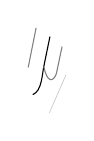
\begin{tikzpicture}[x=.55cm,y=.55cm,line cap=round]
\draw[thin,gray] (0,0) -- (.18,.9);
\draw[thin] (.11,-.63) .. controls (.31,-.55) and (.32,-.18) .. (.36,.02) -- (.50,.70);
\draw[thin,gray] (.36,.02) .. controls (.43,-.35) and (.57,-.36) .. (.65,-.15) -- (.78,.47);
\draw[very thin,gray!50] (.49,-1.05) -- (.87,-.18);
\end{tikzpicture}}
\end{minipage}\hfill\begin{minipage}[t]{.39\linewidth}\vspace{0pt}
\raggedright
Poids et niveaux d'\ignorespaces espaces de cohomologie $\ell$-adiques (base var. quelconque)
\end{minipage}
% archive sheet number: 95
